%! suppress = NonMatchingIf

This section describes the \hardwareversion\ Cow Pi development board, describes the theory of operation for its components, and summarizes the features of its display module.

\subsection{Cow Pi Development Board}\label{subsec:theboard}

The Cow Pi development board consists of a microcontroller board (\mcuboard), a display module (\displaymoduledescription), a $4 \times 4$ matrix keypad, two momentary buttons, two toggleable switches, and two LEDs.
The board is assembled on a \construction; see Figure~\ref{fig:photograph}.

%! suppress = FileNotFound
\begin{figure}
    \centering
    \includegraphics[scale=0.75]{\photograph}
    \caption{A \hardwareversion\ Cow Pi development board.}\label{fig:photograph}
\end{figure}

The toggleable switches are referred to as the \textbf{left switch} and the \textbf{right switch}, and each can be positioned in the left or right position.
When a switch is in the right position, its logic value is high, by way of a pull-up resistor.
When a switch is in the left position, the switch is grounded, and its logic value is low.

The momentary buttons are referred to as the \textbf{left button} and the \textbf{right button}, and each can be pressed (alternatively, in the down position) or unpressed (alternatively, in the up position).
The buttons are normally-open, and so when a button is unpressed, its logic value is high, by way of a pull-up resistor.
When a button is pressed, the button is grounded, and its logic value is low.

The LEDs are referred to as the \textbf{left LED} and the \textbf{right LED}.
\ifboolexpe{bool{nano-form-factor}}{
    The \textbf{left LED} is aliased to the \mcuboard's built-in LED, and some documents may refer to it as the Cow Pi's \textbf{internal LED}.
    \ifdefstring{\construction}{solderless breadboard}{
        Indeed, Arduino-based mark~1 Cow Pis simply use the \mcuboard's built-in LED as the \textbf{left LED} to reduce clutter on the solderless breadboard.
    }{}
    \ifboolexpe{bool{spi}}{
        Note that the \textbf{left LED} may be of limited use in the Cow Pi \cowpiversion\ due to the \mcuboard's \texttt{D13} pin being used for both the \textbf{left} (built-in) \textbf{LED} and also as for the \texttt{SCK} SPI clock signal.
    }{}
    Some documents may refer to the \textbf{right LED} as the Cow Pi's \textbf{external LED}.
}{}
An LED will illuminate when the corresponding microcontroller output is high, and it will deluminate when the corresponding microcontroller output is low.

The matrix keypad is designed to be scanned using the conventional approach of selectively setting the rows' logic values and reading the columns' resulting logic values.
\ifdefstring{\construction}{solderless breadboard}{Note that mark~1 Cow Pis' keypads cannot be accurately scanned if more than two keys are pressed at the same time.
    Further, \textbf{there are no current-limiting protections} (other than the microcontroller's fuses) in place to prevent over-current if simultaneously pressing more than one in the same column shorts a logic-high row to a logic-low row.}{}

The microcontroller communicates with the \displaymoduledescription display module using the
\ifboolexpe{bool{spi}}{Serial Peripheral Interface (SPI) protocol.}{}
\ifboolexpe{bool{i2c}}{Inter-Integrated Circuit (I$^2$C or IIC) protocol, also known as the Two-Wire Interface (TWI) protocol.}{}

\ifboolexpe{bool{spi}}{\ifboolexpe{bool{i2c}}{Figures~\ref{fig:pinouts-nano-spi} and~\ref{fig:pinouts-nano-i2c} show}{Figure~\ref{fig:pinouts-nano-spi} shows}}{\ifboolexpe{bool{i2c}}{Figure~\ref{fig:pinouts-nano-i2c} shows}{}}
which input or output is connected to each of the \mcuboard's pins, as well as which general-purpose input/output register bit corresponds to each pin.

\ifboolexpe{bool{spi}}{
    \begin{figure}[p]
        \centering
        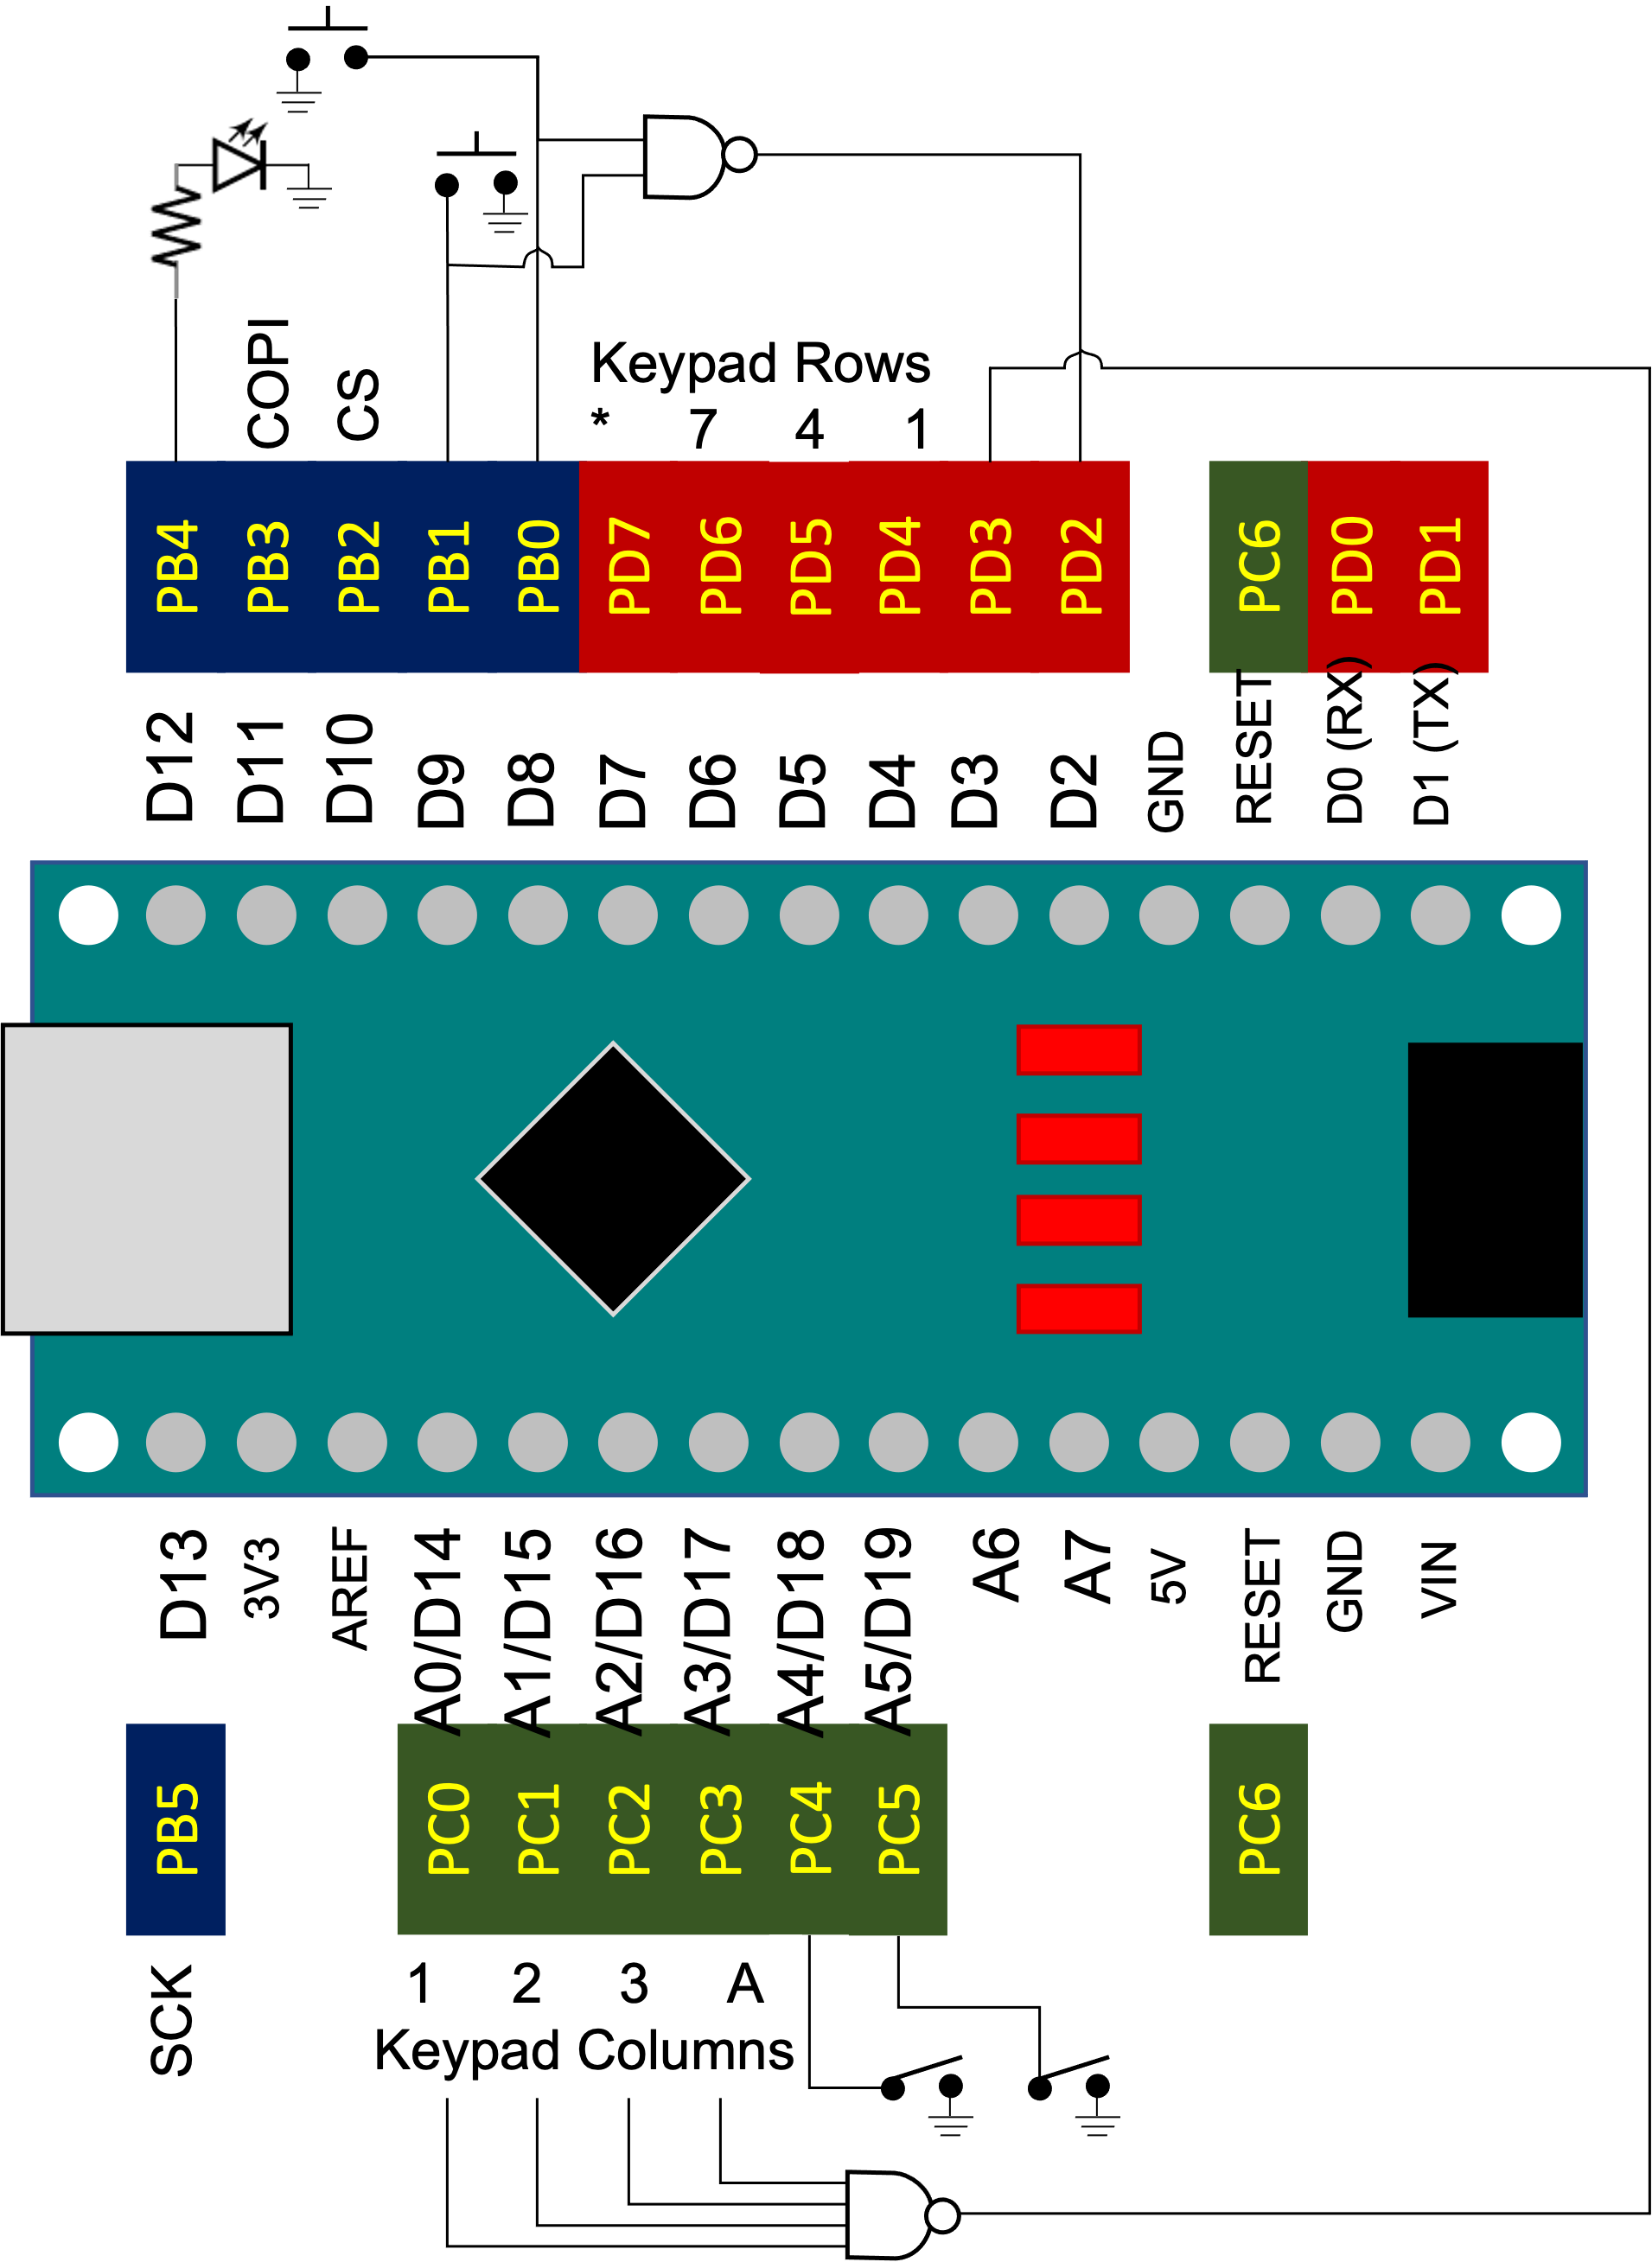
\includegraphics[scale=0.75]{pinouts/nano-spi}
        \caption{Pinout for the \hardwareversion\ Cow Pi development board using \mcuboard and the SPI serial communication protocol.}\label{fig:pinouts-nano-spi}
    \end{figure}
}{}

\ifboolexpe{bool{i2c}}{
    \begin{figure}[p]
        \centering
        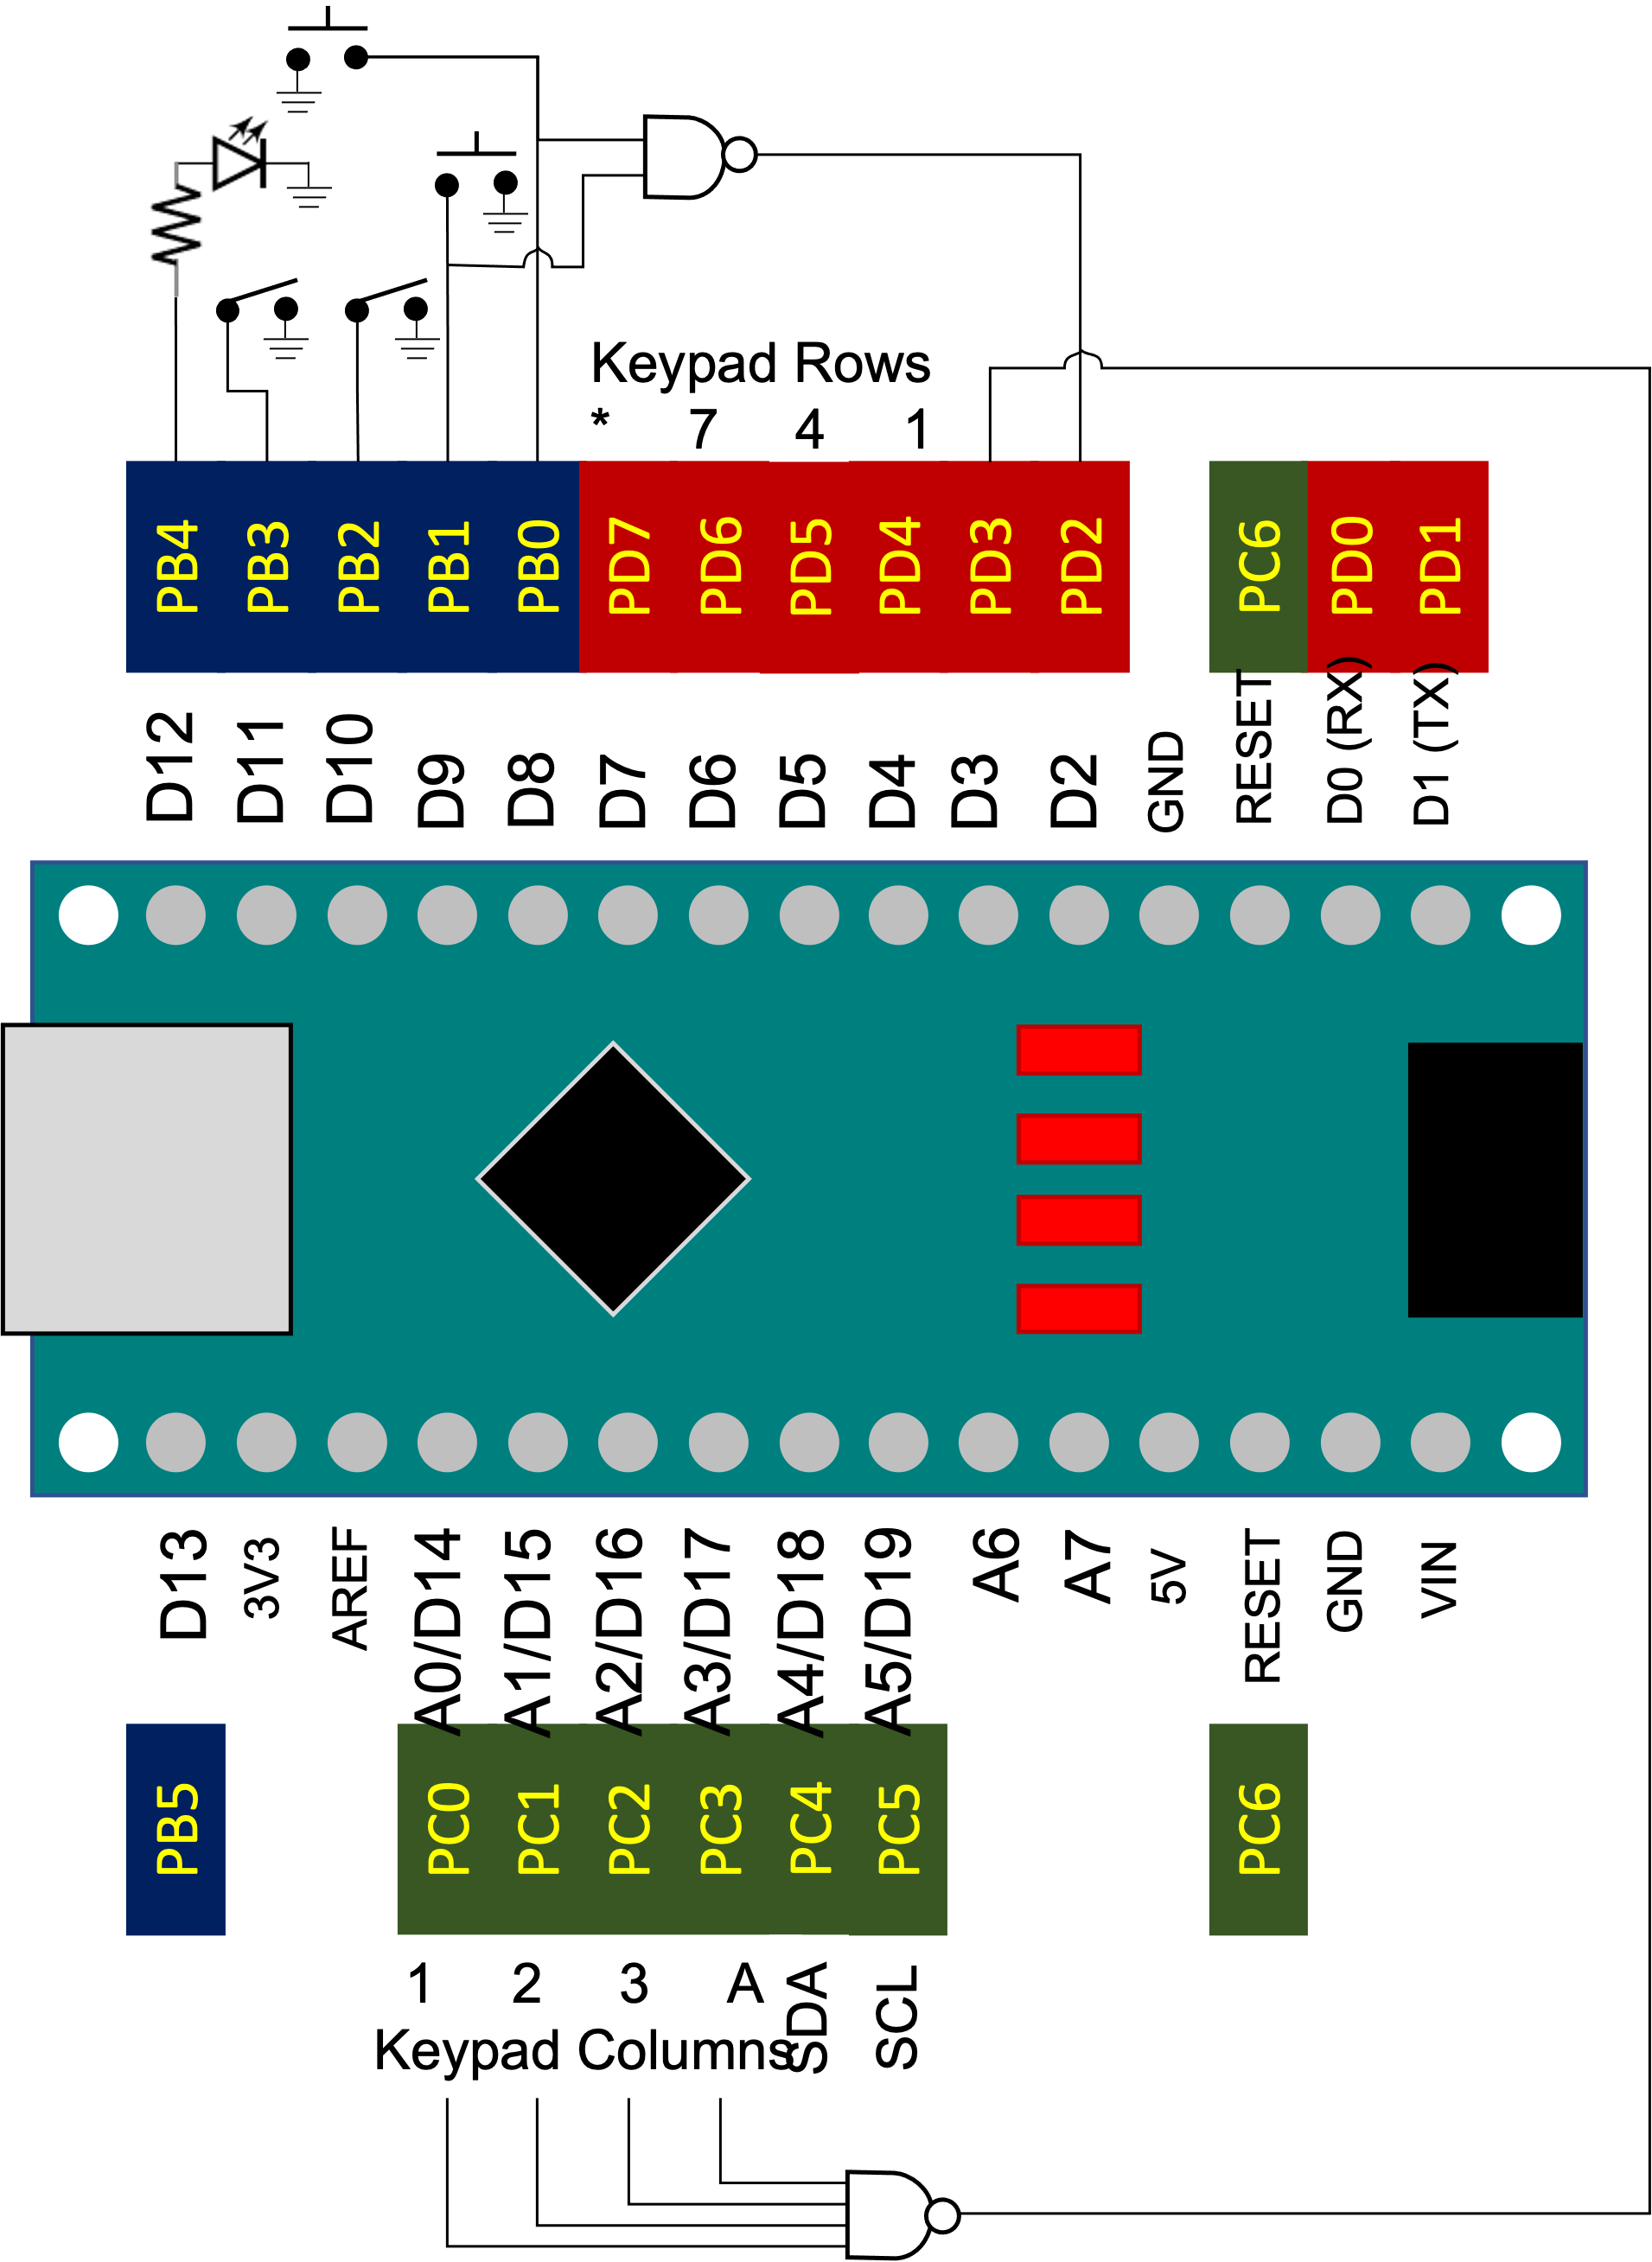
\includegraphics[scale=0.75]{pinouts/nano-i2c}
        \caption{Pinout for a Cow Pi development board using the \mcuboard\ and the I$^2$C serial communication protocol.}\label{fig:pinouts-nano-i2c}
    \end{figure}
}{}

%\subsection{Microcontroller Board}
%
%\subsection{LEDs}
%
%\subsection{Buttons and Switches}
%
\subsection{Matrix Keypad}

\subsubsection{Theory of Operation}

Each key on a matrix keypad is a normally-open, momentary button that resides at the intersection of a row and a column;
see Figure~\ref{fig:basic-keypad}(a).
When pressed, the key closes an electrical connection between that row and column.
On the Cow Pi, each row is connected to an output pin on the \mcuboard, and each column is connected to an input pin with a pull-up resistor.

Because the input pins that the columns are connected to use pull-up resistors, the logic value on these pins will normally read high (boolean 1).
A column will read as logic low (boolean 0) only when it is electrically connected to a row that is set low.
An application developer can take advantage of this by setting all of the rows' pins to logic low (boolean 0);
see Figure~\ref{fig:basic-keypad}(b).
When a key is pressed, its column will then become low.

\begin{figure}[h]
    \hspace{.5in}
    \subfloat[Each key on the keypad is at the intersection of a row and a column.]{
        \centering
        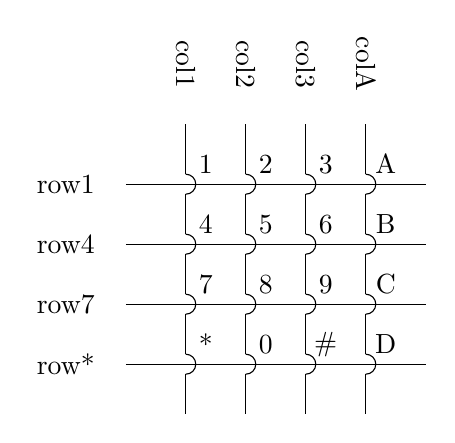
\begin{tikzpicture}[x=.1in, y=.1in]
            \draw (7,10) node {1} +(3,0) node {2} +(6,0) node {3} +(9,0) node {A}
                +(0,-3) node {4} +(3,-3) node {5} +(6,-3) node {6} +(9,-3) node {B}
                +(0,-6) node {7} +(3,-6) node {8} +(6,-6) node {9} +(9,-6) node {C}
                +(0,-9) node {*} +(3,-9) node {0} +(6,-9) node {\#} +(9,-9) node {D};
            \draw (0,9) node {row1} ++(3,0) -- ++(15,0);
            \draw (0,6) node {row4} ++(3,0) -- ++(15,0);
            \draw (0,3) node {row7} ++(3,0) -- ++(15,0);
            \draw (0,0) node {row*} ++(3,0) -- ++(15,0);
            \draw (6,15) node {\rotatebox{-90}{col1}} ++(0,-3) -- ++(0,-2.5) ++(0,-1) -- ++(0,-2) ++(0,-1) -- ++(0,-2) ++(0,-1) -- ++(0,-2) ++(0,-1) -- ++(0,-2);
            \draw (6,9.5) arc [start angle=90, end angle=-90, radius=.5] ++(0,-2) arc [start angle=90, end angle=-90, radius=.5] ++(0,-2) arc [start angle=90, end angle=-90, radius=.5] ++(0,-2) arc [start angle=90, end angle=-90, radius=.5];
            \draw (9,15) node {\rotatebox{-90}{col2}} ++(0,-3) -- ++(0,-2.5) ++(0,-1) -- ++(0,-2) ++(0,-1) -- ++(0,-2) ++(0,-1) -- ++(0,-2) ++(0,-1) -- ++(0,-2);
            \draw (9,9.5) arc [start angle=90, end angle=-90, radius=.5] ++(0,-2) arc [start angle=90, end angle=-90, radius=.5] ++(0,-2) arc [start angle=90, end angle=-90, radius=.5] ++(0,-2) arc [start angle=90, end angle=-90, radius=.5];
            \draw (12,15) node {\rotatebox{-90}{col3}} ++(0,-3) -- ++(0,-2.5) ++(0,-1) -- ++(0,-2) ++(0,-1) -- ++(0,-2) ++(0,-1) -- ++(0,-2) ++(0,-1) -- ++(0,-2);
            \draw (12,9.5) arc [start angle=90, end angle=-90, radius=.5] ++(0,-2) arc [start angle=90, end angle=-90, radius=.5] ++(0,-2) arc [start angle=90, end angle=-90, radius=.5] ++(0,-2) arc [start angle=90, end angle=-90, radius=.5];
            \draw (15,15) node {\rotatebox{-90}{colA}} ++(0,-3) -- ++(0,-2.5) ++(0,-1) -- ++(0,-2) ++(0,-1) -- ++(0,-2) ++(0,-1) -- ++(0,-2) ++(0,-1) -- ++(0,-2);
            \draw (15,9.5) arc [start angle=90, end angle=-90, radius=.5] ++(0,-2) arc [start angle=90, end angle=-90, radius=.5] ++(0,-2) arc [start angle=90, end angle=-90, radius=.5] ++(0,-2) arc [start angle=90, end angle=-90, radius=.5];
        \end{tikzpicture}
    }
    \hfill
    \subfloat[Detecting a keypress is possible by setting each row low and monitoring whether any column becomes low.]{
        \centering
        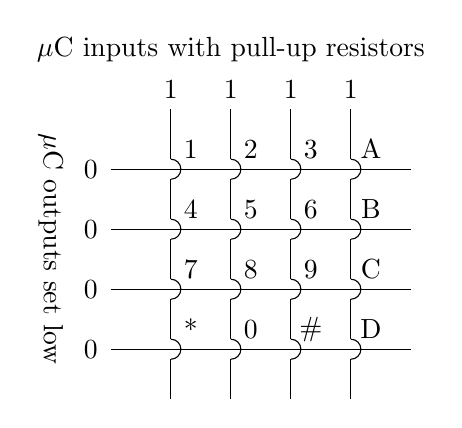
\begin{tikzpicture}[x=.1in, y=.1in]
            \draw (7,10) node {1} +(3,0) node {2} +(6,0) node {3} +(9,0) node {A}
            +(0,-3) node {4} +(3,-3) node {5} +(6,-3) node {6} +(9,-3) node {B}
            +(0,-6) node {7} +(3,-6) node {8} +(6,-6) node {9} +(9,-6) node {C}
            +(0,-9) node {*} +(3,-9) node {0} +(6,-9) node {\#} +(9,-9) node {D};
            \draw (0,5) node {\rotatebox{-90}{$\mu$C outputs set low}};
            \draw (0,9) +(2,0) node {0} ++(3,0) -- ++(15,0);
            \draw (0,6) +(2,0) node {0} ++(3,0) -- ++(15,0);
            \draw (0,3) +(2,0) node {0} ++(3,0) -- ++(15,0);
            \draw (0,0) +(2,0) node {0} ++(3,0) -- ++(15,0);
            \draw (9,15) node {$\mu$C inputs with pull-up resistors};
            \draw (6,15) +(0,-2) node {1} ++(0,-3) -- ++(0,-2.5) ++(0,-1) -- ++(0,-2) ++(0,-1) -- ++(0,-2) ++(0,-1) -- ++(0,-2) ++(0,-1) -- ++(0,-2);
            \draw (6,9.5) arc [start angle=90, end angle=-90, radius=.5] ++(0,-2) arc [start angle=90, end angle=-90, radius=.5] ++(0,-2) arc [start angle=90, end angle=-90, radius=.5] ++(0,-2) arc [start angle=90, end angle=-90, radius=.5];
            \draw (9,15) +(0,-2) node {1} ++(0,-3) -- ++(0,-2.5) ++(0,-1) -- ++(0,-2) ++(0,-1) -- ++(0,-2) ++(0,-1) -- ++(0,-2) ++(0,-1) -- ++(0,-2);
            \draw (9,9.5) arc [start angle=90, end angle=-90, radius=.5] ++(0,-2) arc [start angle=90, end angle=-90, radius=.5] ++(0,-2) arc [start angle=90, end angle=-90, radius=.5] ++(0,-2) arc [start angle=90, end angle=-90, radius=.5];
            \draw (12,15) +(0,-2) node {1} ++(0,-3) -- ++(0,-2.5) ++(0,-1) -- ++(0,-2) ++(0,-1) -- ++(0,-2) ++(0,-1) -- ++(0,-2) ++(0,-1) -- ++(0,-2);
            \draw (12,9.5) arc [start angle=90, end angle=-90, radius=.5] ++(0,-2) arc [start angle=90, end angle=-90, radius=.5] ++(0,-2) arc [start angle=90, end angle=-90, radius=.5] ++(0,-2) arc [start angle=90, end angle=-90, radius=.5];
            \draw (15,15) +(0,-2) node {1} ++(0,-3) -- ++(0,-2.5) ++(0,-1) -- ++(0,-2) ++(0,-1) -- ++(0,-2) ++(0,-1) -- ++(0,-2) ++(0,-1) -- ++(0,-2);
            \draw (15,9.5) arc [start angle=90, end angle=-90, radius=.5] ++(0,-2) arc [start angle=90, end angle=-90, radius=.5] ++(0,-2) arc [start angle=90, end angle=-90, radius=.5] ++(0,-2) arc [start angle=90, end angle=-90, radius=.5];
        \end{tikzpicture}
    }
    \hspace{.5in}
    \caption{Preparing a matrix keypad to detect keypresses.} \label{fig:basic-keypad}
\end{figure}

A keypress, thus, can be detected based on the values read from the columns' pins.
A pin-change interrupt that is triggered by a change on the columns' pins can be used to indicate that a key has been pressed;
however, for the \hardwareversion~Cow Pi, it is probably easier to use an external interrupt that is triggered by a change in the output of the NAND gate that is also connected to the keypad's columns (see Section~\ref{sec:Interrupts}).
As an alternative to using an interrupt, an application programmer can poll the four columns' pins.
If, collectively, they produce the bit vector 0xF, then no key is being pressed;
however, if the bit vector is anything other than 0xF, then at least one key is being pressed.

Once it has been determined that a key is pressed, code that scans the keypad should execute.
If every row is made logic-high \textit{except} for one row, then the code can determine whether the key that was pressed is in that row.
For example, as shown in Figure~\ref{fig:scanning-keypad}(a), if the ``8'' key is pressed and ``row4'' is the only logic-low row, then the column bit vector is 0xF, and so the pressed key is not in that row.
But, as shown in Figure~\ref{fig:scanning-keypad}(b), if ``row7'' is the only logic-low row, then the column bit vector is not 0xF, and so the pressed key is in that row;
moreover, because ``col2'' is now logic-low, the code can establish that the pressed key is at the intersection of ``row7'' and ``col2,'' \textit{i.e.}, the ``8'' key.

\begin{figure}[h]
    \hspace{.5in}
    \subfloat[Examining a row that does not have a pressed key.]{
        \centering
        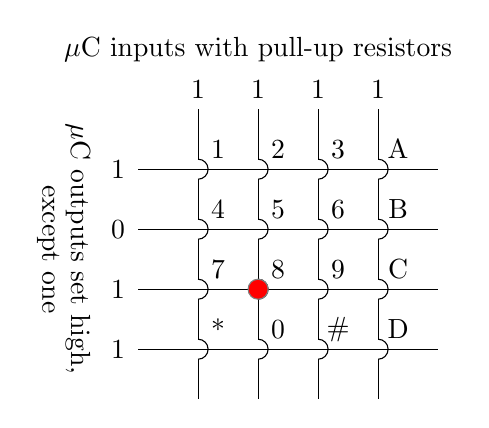
\begin{tikzpicture}[x=.1in, y=.1in]
            \draw (7,10) node {1} +(3,0) node {2} +(6,0) node {3} +(9,0) node {A}
            +(0,-3) node {4} +(3,-3) node {5} +(6,-3) node {6} +(9,-3) node {B}
            +(0,-6) node {7} +(3,-6) node {8} +(6,-6) node {9} +(9,-6) node {C}
            +(0,-9) node {*} +(3,-9) node {0} +(6,-9) node {\#} +(9,-9) node {D};
            \draw (0,5) node {\rotatebox{-90}{$\mu$C outputs set high,}};
            \draw (-1.5,5) node {\rotatebox{-90}{except one}};
            \draw (0,9) +(2,0) node {1} ++(3,0) -- ++(15,0);
            \draw (0,6) +(2,0) node {0} ++(3,0) -- ++(15,0);
            \draw (0,3) +(2,0) node {1} ++(3,0) -- ++(15,0);
            \draw (0,0) +(2,0) node {1} ++(3,0) -- ++(15,0);
            \draw (9,15) node {$\mu$C inputs with pull-up resistors};
            \draw (6,15) +(0,-2) node {1} ++(0,-3) -- ++(0,-2.5) ++(0,-1) -- ++(0,-2) ++(0,-1) -- ++(0,-2) ++(0,-1) -- ++(0,-2) ++(0,-1) -- ++(0,-2);
            \draw (6,9.5) arc [start angle=90, end angle=-90, radius=.5] ++(0,-2) arc [start angle=90, end angle=-90, radius=.5] ++(0,-2) arc [start angle=90, end angle=-90, radius=.5] ++(0,-2) arc [start angle=90, end angle=-90, radius=.5];
            \draw (9,15) +(0,-2) node {1} ++(0,-3) -- ++(0,-2.5) ++(0,-1) -- ++(0,-2) ++(0,-1) -- ++(0,-2) ++(0,-1) -- ++(0,-2) ++(0,-1) -- ++(0,-2);
            \draw (9,9.5) arc [start angle=90, end angle=-90, radius=.5] ++(0,-2) arc [start angle=90, end angle=-90, radius=.5] ++(0,-2) arc [start angle=90, end angle=-90, radius=.5] ++(0,-2) arc [start angle=90, end angle=-90, radius=.5];
            \draw (12,15) +(0,-2) node {1} ++(0,-3) -- ++(0,-2.5) ++(0,-1) -- ++(0,-2) ++(0,-1) -- ++(0,-2) ++(0,-1) -- ++(0,-2) ++(0,-1) -- ++(0,-2);
            \draw (12,9.5) arc [start angle=90, end angle=-90, radius=.5] ++(0,-2) arc [start angle=90, end angle=-90, radius=.5] ++(0,-2) arc [start angle=90, end angle=-90, radius=.5] ++(0,-2) arc [start angle=90, end angle=-90, radius=.5];
            \draw (15,15) +(0,-2) node {1} ++(0,-3) -- ++(0,-2.5) ++(0,-1) -- ++(0,-2) ++(0,-1) -- ++(0,-2) ++(0,-1) -- ++(0,-2) ++(0,-1) -- ++(0,-2);
            \draw (15,9.5) arc [start angle=90, end angle=-90, radius=.5] ++(0,-2) arc [start angle=90, end angle=-90, radius=.5] ++(0,-2) arc [start angle=90, end angle=-90, radius=.5] ++(0,-2) arc [start angle=90, end angle=-90, radius=.5];
            \draw[gray, fill=red] (9,3) circle (.5);
        \end{tikzpicture}
    }
    \hfill
    \subfloat[Examining a row that does have a pressed key.]{
        \centering
        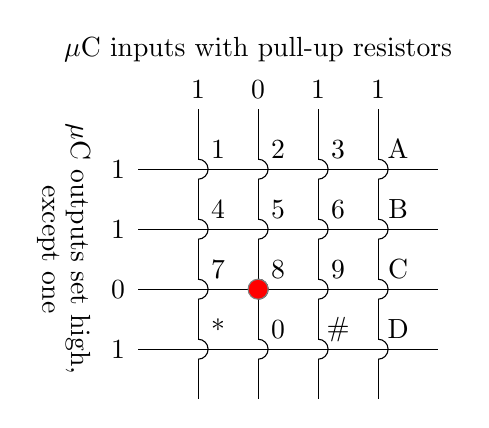
\begin{tikzpicture}[x=.1in, y=.1in]
            \draw (7,10) node {1} +(3,0) node {2} +(6,0) node {3} +(9,0) node {A}
            +(0,-3) node {4} +(3,-3) node {5} +(6,-3) node {6} +(9,-3) node {B}
            +(0,-6) node {7} +(3,-6) node {8} +(6,-6) node {9} +(9,-6) node {C}
            +(0,-9) node {*} +(3,-9) node {0} +(6,-9) node {\#} +(9,-9) node {D};
            \draw (0,5) node {\rotatebox{-90}{$\mu$C outputs set high,}};
            \draw (-1.5,5) node {\rotatebox{-90}{except one}};
            \draw (0,9) +(2,0) node {1} ++(3,0) -- ++(15,0);
            \draw (0,6) +(2,0) node {1} ++(3,0) -- ++(15,0);
            \draw (0,3) +(2,0) node {0} ++(3,0) -- ++(15,0);
            \draw (0,0) +(2,0) node {1} ++(3,0) -- ++(15,0);
            \draw (9,15) node {$\mu$C inputs with pull-up resistors};
            \draw (6,15) +(0,-2) node {1} ++(0,-3) -- ++(0,-2.5) ++(0,-1) -- ++(0,-2) ++(0,-1) -- ++(0,-2) ++(0,-1) -- ++(0,-2) ++(0,-1) -- ++(0,-2);
            \draw (6,9.5) arc [start angle=90, end angle=-90, radius=.5] ++(0,-2) arc [start angle=90, end angle=-90, radius=.5] ++(0,-2) arc [start angle=90, end angle=-90, radius=.5] ++(0,-2) arc [start angle=90, end angle=-90, radius=.5];
            \draw (9,15) +(0,-2) node {0} ++(0,-3) -- ++(0,-2.5) ++(0,-1) -- ++(0,-2) ++(0,-1) -- ++(0,-2) ++(0,-1) -- ++(0,-2) ++(0,-1) -- ++(0,-2);
            \draw (9,9.5) arc [start angle=90, end angle=-90, radius=.5] ++(0,-2) arc [start angle=90, end angle=-90, radius=.5] ++(0,-2) arc [start angle=90, end angle=-90, radius=.5] ++(0,-2) arc [start angle=90, end angle=-90, radius=.5];
            \draw (12,15) +(0,-2) node {1} ++(0,-3) -- ++(0,-2.5) ++(0,-1) -- ++(0,-2) ++(0,-1) -- ++(0,-2) ++(0,-1) -- ++(0,-2) ++(0,-1) -- ++(0,-2);
            \draw (12,9.5) arc [start angle=90, end angle=-90, radius=.5] ++(0,-2) arc [start angle=90, end angle=-90, radius=.5] ++(0,-2) arc [start angle=90, end angle=-90, radius=.5] ++(0,-2) arc [start angle=90, end angle=-90, radius=.5];
            \draw (15,15) +(0,-2) node {1} ++(0,-3) -- ++(0,-2.5) ++(0,-1) -- ++(0,-2) ++(0,-1) -- ++(0,-2) ++(0,-1) -- ++(0,-2) ++(0,-1) -- ++(0,-2);
            \draw (15,9.5) arc [start angle=90, end angle=-90, radius=.5] ++(0,-2) arc [start angle=90, end angle=-90, radius=.5] ++(0,-2) arc [start angle=90, end angle=-90, radius=.5] ++(0,-2) arc [start angle=90, end angle=-90, radius=.5];
            \draw[gray, fill=red] (9,3) circle (.5);
        \end{tikzpicture}
    }
    \hspace{.5in}
    \caption{Scanning a matrix keypad. The red dot indicates which key is being pressed.} \label{fig:scanning-keypad}
\end{figure}

After the code has determined which row and column the pressed key is on, it can return a value or assign a value to a variable accordingly.
This might be a \lstinline{char} corresponding to the character on the key's face, as is the case for \function{cowpi_get_keypress} (Section~\ref{subsec:ScannedInputs}).
Or this might be an \lstinline{int} corresponding to the value of the numeral on the key's face.
Or this might even be some value unrelated to whatever is printed on the key's face.

\subsubsection{Scanning the Keypad}

There are a few options for obtaining the value corresponding to a key that is pressed on the keypad.
The most efficient for a simple application is to use a lookup table.
For example, if you need to return a character that corresponds to the face value of the key that was pressed, then the lookup table would be:
\[
    keys \gets
    \left(\begin{array}{cccc}
              '1' & '2' & '3' & 'A' \\
              '4' & '5' & '6' & 'B' \\
              '7' & '8' & '9' & 'C' \\
              '*' & '0' & '\#' & 'D'
    \end{array}\right)
\]

If the keypad is wired to the \mcuboard\ such that four contiguous output pins are connected to the rows and four contiguous input pins are connected to the columns (as is the case for the Cow Pi), then this pseudocode will scan the keypad and determine which key, if any, is pressed:
Note that this pseudocode will report at most one key pressed;
it would have to be modified to report multiple keys pressed.
(This software limitation is not a limitation for mark~1 Cow Pis, as mark~1 Cow Pis have a hardware limitation:
their keypads have no protection against shorting power to ground when two keys are pressed simultaneously.)

\begin{lstlisting}[language=pascal,basicstyle=\rmfamily\footnotesize,literate={:=}{{$\gets$}}1 {<=}{{$\leq$}}1 {>=}{{$\geq$}}1 {<>}{{$\neq$}}1 {->}{{$\succ$}}1, escapechar=`]
for each row:
    row_bit_vector := 0b1111    (* set all rows to 1 *)
    row_bit_vector(row) := 0    (* except the row we're currently examining *)
    wait at least one microcontroller clock cycle   `\label{line:keypad_delay}`
    for each column:
        if (column_bit_vector(column) = 0):
            key_pressed := keys(row,column)
row_bit_vector := 0b0000        (* set all rows to 0 to detect the next keypress *)
\end{lstlisting}

The delay shown in line~\ref{line:keypad_delay} is sometimes, but not always necessary.
There is a slight delay between setting a pin's output value and being able to detect the change by reading a different pin's input value.
Some realizations of the pseudocode attempt to read the change before it can be read reliably;
this usually manifests as one of the keypad's columns not being readable.
The fix is to introduce a delay of at least one clock cycle (strictly speaking, one clock cycle is more than enough, but a shorter delay is not possible).
This could be managed by introducing a delay based on the microcontroller's clock cycle, using the AVR-libc \function{_NOP()} or \function{_delay_loop_1()} functions,\cite{avrNOP}\cite{avrDelayBasic} to be able to introduce a delay of exactly one or three clock cycles (\function{_NOP()} or \function{_delay_loop_1(1)}, respectively),
or this could be managed by introducing a 1$\mu$s delay using the Arduino core library's \function{delayMicroseconds()} function,\cite{arduinoDelay} which is portable across all devices using the Arduino toolchain.

\subsection{Display Module}

The display module used in the \hardwareversion~Cow Pi is a \displaymoduledescription.
A full description of its control signals can be found in the HD44780U datasheet;\cite{lcd1602}
however, the CowPi library's functions handles these control signals -- see Section~\ref{subsec:DisplayModules}.
If a function to send a halfbyte to the display module is registered, either the CowPi library's default implementation or your own (Section~\ref{subsubsec:send_halfbyte}), then you do not need to manage the control signals.

Displaying useful information on the display module does require some awareness of the dipslay module's characteristics.
As previously stated, the display module can display up to 32 characters, 16 characters on each of two rows.
When sending these characters using the library's \hyperlink{function:cowpi_lcd1602_place_character}{\function{cowpi_lcd1602_place_character()}} or \hyperlink{function:cowpi_lcd1602_send_character}{\function{cowpi_lcd1602_send_character()}} functions, you typically can use standard ASCII characters.
Specifically, if the \lstinline{character} argument is in the range 0x20--0x7D, then the corresponding ASCII character will be displayed.
For the characters displayed when the argument is 0x7E, 0x7F, or in the range 0xA1--0xFF, see Table~4 of the HD44780U datasheet.\cite{lcd1602}
Up to eight custom characters can also be created; see the \hyperlink{function:cowpi_lcd1602_create_character}{\function{cowpi_lcd1602_create_character()}} function and the \textit{lcd1602\_custom\_characters} example program described in Section~\ref{subsec:CustomCharacters}.

While there are 16 characters displayed per row, the display module has memory addresses for 40 characters per row.
The base address of the top row is 0x00, and the base address of the bottom row is 0x40.
Initially, the characters at addresses 0x00--0x0F and 0x40--0x4F are displayed, as shown in Figure~\ref{fig:initial-display}.

\begin{figure}[t]
    \centering
    \tiny
    \begin{tikzpicture}[x=.1in, y=.1in, square/.style={regular polygon,regular polygon sides=4,inner sep=0,minimum size=1.2cm}]
        \node at (0,0) [square,draw,anchor=west] (0x00) {0x00};
        \node at (0x00.east) [square,draw,anchor=west] (0x01) {0x01};
        \node at (0x01.east) [square,draw,anchor=west] (0x02) {0x02};
        \node at (0x02.east) [square,draw,anchor=west] (0x03) {0x03};
        \node at (0x03.east) [square,draw,anchor=west] (0x04) {0x04};
        \node at (0x04.east) [square,draw,anchor=west] (0x05) {0x05};
        \node at (0x05.east) [square,draw,anchor=west] (0x06) {0x06};
        \node at (0x06.east) [square,draw,anchor=west] (0x07) {0x07};
        \node at (0x07.east) [square,draw,anchor=west] (0x08) {0x08};
        \node at (0x08.east) [square,draw,anchor=west] (0x09) {0x09};
        \node at (0x09.east) [square,draw,anchor=west] (0x0A) {0x0A};
        \node at (0x0A.east) [square,draw,anchor=west] (0x0B) {0x0B};
        \node at (0x0B.east) [square,draw,anchor=west] (0x0C) {0x0C};
        \node at (0x0C.east) [square,draw,anchor=west] (0x0D) {0x0D};
        \node at (0x0D.east) [square,draw,anchor=west] (0x0E) {0x0E};
        \node at (0x0E.east) [square,draw,anchor=west] (0x0F) {0x0F};
        \node at (0x00.south) [square,draw,anchor=north] (0x40) {0x40};
        \node at (0x40.east) [square,draw,anchor=west] (0x41) {0x41};
        \node at (0x41.east) [square,draw,anchor=west] (0x42) {0x42};
        \node at (0x42.east) [square,draw,anchor=west] (0x43) {0x43};
        \node at (0x43.east) [square,draw,anchor=west] (0x44) {0x44};
        \node at (0x44.east) [square,draw,anchor=west] (0x45) {0x45};
        \node at (0x45.east) [square,draw,anchor=west] (0x46) {0x46};
        \node at (0x46.east) [square,draw,anchor=west] (0x47) {0x47};
        \node at (0x47.east) [square,draw,anchor=west] (0x48) {0x48};
        \node at (0x48.east) [square,draw,anchor=west] (0x49) {0x49};
        \node at (0x49.east) [square,draw,anchor=west] (0x4A) {0x4A};
        \node at (0x4A.east) [square,draw,anchor=west] (0x4B) {0x4B};
        \node at (0x4B.east) [square,draw,anchor=west] (0x4C) {0x4C};
        \node at (0x4C.east) [square,draw,anchor=west] (0x4D) {0x4D};
        \node at (0x4D.east) [square,draw,anchor=west] (0x4E) {0x4E};
        \node at (0x4E.east) [square,draw,anchor=west] (0x4F) {0x4F};
        \draw[blue,ultra thick] (0x00.north west) rectangle (0x4F.south east);
        \node at (0x0F.east) [square,draw,anchor=west] (0x10) {0x10};
        \node at (0x4F.east) [square,draw,anchor=west] (0x50) {0x50};
        \node at (0x10.east) [square,draw,anchor=west] (0x11) {0x11};
        \node at (0x50.east) [square,draw,anchor=west] (0x51) {0x51};
        \node at (0x11.east) [white,square,draw,anchor=west] (dots0) {$\dots$};
        \node at (0x51.east) [white,square,draw,anchor=west] (dots1) {$\dots$};
        \draw (dots0.center) node {$\dots$};
        \draw (dots1.center) node {$\dots$};
        \node at (dots0.east) [square,draw,anchor=west] (0x27) {0x27};
        \node at (dots1.east) [square,draw,anchor=west] (0x67) {0x67};
    \end{tikzpicture}
    \caption{Initially, the characters at addresses 0x00--0x0F and 0x40--0x4F are displayed. The black squares are character memory locations; the blue rectangle shows which characters are displayed.} \label{fig:initial-display}
\end{figure}

The displayed addresses can shift to the left or to the right.
Normally the display will not shift when a character is displayed; however, the display can be configured to shift with each new character added.
This is achieved by changing the entry mode with the \hyperlink{function:cowpi_lcd1602_send_command}{\function{cowpi_lcd1602_send_command()}} function.
Alternatively, the display can be explicitly shifted, regardless of the entry mode. If the \hyperlink{function:cowpi_lcd1602_send_command}{\function{cowpi_lcd1602_send_command()}} function is used so send the \lstinline{LCDSHIFT_DISPLAYLEFT} or the \lstinline{LCD_DISPLAY_RIGHT} command, then the display will shift to the left or to the right accordingly.

For example, if the display is shifted to the left from its initial configuration, then the characters at addresses 0x01--0x10 and 0x41--0x50 are displayed, as shown in Figure~\ref{fig:shiftleft-display}.

\begin{figure}[t]
    \centering
    \tiny
    \begin{tikzpicture}[x=.1in, y=.1in, square/.style={regular polygon,regular polygon sides=4,inner sep=0,minimum size=1.2cm}]
        \node at (0,0) [square,draw,anchor=west] (0x01) {0x01};
        \node at (0x01.east) [square,draw,anchor=west] (0x02) {0x02};
        \node at (0x02.east) [square,draw,anchor=west] (0x03) {0x03};
        \node at (0x03.east) [square,draw,anchor=west] (0x04) {0x04};
        \node at (0x04.east) [square,draw,anchor=west] (0x05) {0x05};
        \node at (0x05.east) [square,draw,anchor=west] (0x06) {0x06};
        \node at (0x06.east) [square,draw,anchor=west] (0x07) {0x07};
        \node at (0x07.east) [square,draw,anchor=west] (0x08) {0x08};
        \node at (0x08.east) [square,draw,anchor=west] (0x09) {0x09};
        \node at (0x09.east) [square,draw,anchor=west] (0x0A) {0x0A};
        \node at (0x0A.east) [square,draw,anchor=west] (0x0B) {0x0B};
        \node at (0x0B.east) [square,draw,anchor=west] (0x0C) {0x0C};
        \node at (0x0C.east) [square,draw,anchor=west] (0x0D) {0x0D};
        \node at (0x0D.east) [square,draw,anchor=west] (0x0E) {0x0E};
        \node at (0x0E.east) [square,draw,anchor=west] (0x0F) {0x0F};
        \node at (0x01.south) [square,draw,anchor=north] (0x41) {0x41};
        \node at (0x41.east) [square,draw,anchor=west] (0x42) {0x42};
        \node at (0x42.east) [square,draw,anchor=west] (0x43) {0x43};
        \node at (0x43.east) [square,draw,anchor=west] (0x44) {0x44};
        \node at (0x44.east) [square,draw,anchor=west] (0x45) {0x45};
        \node at (0x45.east) [square,draw,anchor=west] (0x46) {0x46};
        \node at (0x46.east) [square,draw,anchor=west] (0x47) {0x47};
        \node at (0x47.east) [square,draw,anchor=west] (0x48) {0x48};
        \node at (0x48.east) [square,draw,anchor=west] (0x49) {0x49};
        \node at (0x49.east) [square,draw,anchor=west] (0x4A) {0x4A};
        \node at (0x4A.east) [square,draw,anchor=west] (0x4B) {0x4B};
        \node at (0x4B.east) [square,draw,anchor=west] (0x4C) {0x4C};
        \node at (0x4C.east) [square,draw,anchor=west] (0x4D) {0x4D};
        \node at (0x4D.east) [square,draw,anchor=west] (0x4E) {0x4E};
        \node at (0x4E.east) [square,draw,anchor=west] (0x4F) {0x4F};
        \node at (0x0F.east) [square,draw,anchor=west] (0x10) {0x10};
        \node at (0x4F.east) [square,draw,anchor=west] (0x50) {0x50};
        \draw[blue,ultra thick] (0x01.north west) rectangle (0x50.south east);
        \node at (0x10.east) [square,draw,anchor=west] (0x11) {0x11};
        \node at (0x50.east) [square,draw,anchor=west] (0x51) {0x51};
        \node at (0x11.east) [square,draw,anchor=west] (0x12) {0x12};
        \node at (0x51.east) [square,draw,anchor=west] (0x52) {0x52};
        \node at (0x12.east) [white,square,draw,anchor=west] (dots0) {$\dots$};
        \node at (0x52.east) [white,square,draw,anchor=west] (dots1) {$\dots$};
        \draw (dots0.center) node {$\dots$};
        \draw (dots1.center) node {$\dots$};
        \node at (dots0.east) [square,draw,anchor=west] (0x27) {0x27};
        \node at (dots1.east) [square,draw,anchor=west] (0x67) {0x67};
        \node at (0x27.east) [square,draw,anchor=west] (0x00) {0x00};
        \node at (0x67.east) [square,draw,anchor=west] (0x00) {0x00};
    \end{tikzpicture}
    \caption{After shifting the display to the left, the characters at addresses 0x01--0x10 and 0x41--0x50 are displayed. The black squares are character memory locations; the blue rectangle shows which characters are displayed.} \label{fig:shiftleft-display}
\end{figure}

If, when shifting, one ``end'' of the rows or the other is passed, then the display ``wraps'' around, displaying some characters at both ends of the rows' addresses.
For example, if the display is shifted to the right from its initial configuration, then the characters at addresses 0x27, 0x00--0x0E and 0x67, 0x40--0x4E are displayed, as shown in Figure~\ref{fig:shiftright-display}.

\begin{figure}[h]
    \centering
    \tiny
    \begin{tikzpicture}[x=.1in, y=.1in, square/.style={regular polygon,regular polygon sides=4,inner sep=0,minimum size=1.2cm}]
        \node at (0,0) [square,draw,anchor=west] (0x27) {0x27};
        \node at (0x27.east) [square,draw,anchor=west] (0x00) {0x00};
        \node at (0x00.east) [square,draw,anchor=west] (0x01) {0x01};
        \node at (0x01.east) [square,draw,anchor=west] (0x02) {0x02};
        \node at (0x02.east) [square,draw,anchor=west] (0x03) {0x03};
        \node at (0x03.east) [square,draw,anchor=west] (0x04) {0x04};
        \node at (0x04.east) [square,draw,anchor=west] (0x05) {0x05};
        \node at (0x05.east) [square,draw,anchor=west] (0x06) {0x06};
        \node at (0x06.east) [square,draw,anchor=west] (0x07) {0x07};
        \node at (0x07.east) [square,draw,anchor=west] (0x08) {0x08};
        \node at (0x08.east) [square,draw,anchor=west] (0x09) {0x09};
        \node at (0x09.east) [square,draw,anchor=west] (0x0A) {0x0A};
        \node at (0x0A.east) [square,draw,anchor=west] (0x0B) {0x0B};
        \node at (0x0B.east) [square,draw,anchor=west] (0x0C) {0x0C};
        \node at (0x0C.east) [square,draw,anchor=west] (0x0D) {0x0D};
        \node at (0x0D.east) [square,draw,anchor=west] (0x0E) {0x0E};
        \node at (0x27.south) [square,draw,anchor=north] (0x67) {0x67};
        \node at (0x67.east) [square,draw,anchor=west] (0x40) {0x40};
        \node at (0x40.east) [square,draw,anchor=west] (0x41) {0x41};
        \node at (0x41.east) [square,draw,anchor=west] (0x42) {0x42};
        \node at (0x42.east) [square,draw,anchor=west] (0x43) {0x43};
        \node at (0x43.east) [square,draw,anchor=west] (0x44) {0x44};
        \node at (0x44.east) [square,draw,anchor=west] (0x45) {0x45};
        \node at (0x45.east) [square,draw,anchor=west] (0x46) {0x46};
        \node at (0x46.east) [square,draw,anchor=west] (0x47) {0x47};
        \node at (0x47.east) [square,draw,anchor=west] (0x48) {0x48};
        \node at (0x48.east) [square,draw,anchor=west] (0x49) {0x49};
        \node at (0x49.east) [square,draw,anchor=west] (0x4A) {0x4A};
        \node at (0x4A.east) [square,draw,anchor=west] (0x4B) {0x4B};
        \node at (0x4B.east) [square,draw,anchor=west] (0x4C) {0x4C};
        \node at (0x4C.east) [square,draw,anchor=west] (0x4D) {0x4D};
        \node at (0x4D.east) [square,draw,anchor=west] (0x4E) {0x4E};
        \draw[blue,ultra thick] (0x27.north west) rectangle (0x4E.south east);
        \node at (0x0E.east) [square,draw,anchor=west] (0x0F) {0x0F};
        \node at (0x4E.east) [square,draw,anchor=west] (0x4F) {0x4F};
        \node at (0x0F.east) [square,draw,anchor=west] (0x10) {0x10};
        \node at (0x4F.east) [square,draw,anchor=west] (0x50) {0x50};
        \node at (0x10.east) [white,square,draw,anchor=west] (dots0) {$\dots$};
        \node at (0x50.east) [white,square,draw,anchor=west] (dots1) {$\dots$};
        \draw (dots0.center) node {$\dots$};
        \draw (dots1.center) node {$\dots$};
        \node at (dots0.east) [square,draw,anchor=west] (0x26) {0x26};
        \node at (dots1.east) [square,draw,anchor=west] (0x66) {0x66};
    \end{tikzpicture}
    \caption{When shifting, the display ``wraps'' around the rows' addresses. The black squares are character memory locations; the blue rectangle shows which characters are displayed.} \label{fig:shiftright-display}
\end{figure}


